\section{Implications for the optimization of \acs{WCA}}

In this section, we will discuss the implications of the methodology for the optimization of \gls{WCA} applications, in particular when employing the experimental results and the improved model of human timings discussed in \cref{sec:extendingmethodology}.
The discussion presented here is a summarized version of what \cref{paper:olguinmunoz2023realistic} exposes.

\todo[inline]{Do we need more experiments?}

\subsection{Implications with respect to task completion times}

The term \emph{task completion time}, in the context of \gls{WCA}, will refer to the time it takes a user to work their way through the task presented by an assistant application.
In \cref{paper:olguinmunoz2023realistic} we refer interchangeably to task completion times as application lifetimes.
This metric directly relates to system resource and energy consumption --- longer task completion times mean that the system is occupied for longer and thus uses more resources.
It thus presents a relatively straightforward yet interesting starting point for the study of the implications of the model on the optimization of \gls{WCA} systems.

The main question we aim to ask relates to the consequences of using our model of human timing behaviors versus using a less realistic approximation.
Specifically, we aim to quantify the difference in task completion times when using the realistic compared to a baseline model which does not take into consideration higher order effects on execution times.
Our reference baseline corresponds to a first order approximation to empirical execution time modeling, using an \gls{exGaussian} distribution fitted to \emph{all} the data points from \cref{paper:olguinmunoz2021impact} (without any grouping whatsoever) which is randomly sampled to obtain execution time values.

\begin{figure}
    \centering
    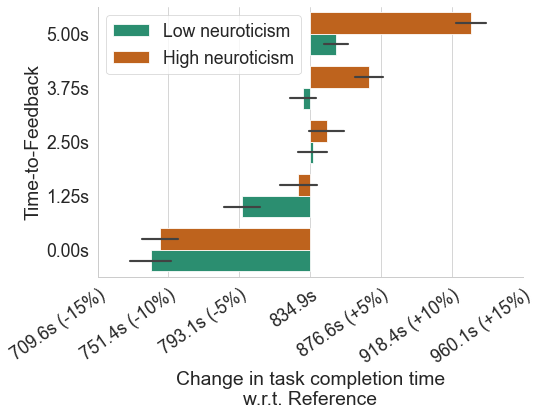
\includegraphics[height=13em]{Figs/2023EdgeDroid2/task_durations_diff}
    \caption{Difference in task completion times of the realistic model with respect to the reference baseline.
    Bars indicate \SI{95}{\percent} \glspl{CI}.}\label{fig:taskcompletiontimesdiff}
\end{figure}

In \cref{fig:taskcompletiontimesdiff} we present the results of an initial, simulated, exploration of the difference in task execution times generated by the model with respect to the baseline.
A \num{100}-step task is simulated at five different, constant \glspl{TTF}; baseline total duration was, on average, \SI{834.87}{\second}.


\subsection{Implications with respect to number of samples per step}

\subsection{Implications with respect to raw energy consumption}
